\documentclass[10pt]{beamer}

\usepackage{fontspec}
\usepackage{xunicode}
\usepackage{xltxtra}
\setsansfont{FreeSans}
\setmonofont{DejaVuSansMono}

\usepackage{listings}
\usepackage{textpos}
\usepackage{tikz}
\usepackage{minted}

\setbeamertemplate{footline}[frame]
\setbeamertemplate{items}[default]
\usetheme{Warsaw}
\usecolortheme{seahorse}
\setbeamertemplate{itemize items}[default]
\setbeamertemplate{navigation symbols}{}
\setbeamertemplate{footline}[frame number]
\lstset{columns=fixed}
\setbeamerfont*{block body}{series=\tt}
\definecolor{lightgray}{rgb}{0.9,0.9,0.9}
\definecolor{midgray}{rgb}{0.5,0.5,0.5}

\usetikzlibrary{arrows,positioning}
\tikzset{
    %Define standard arrow tip
    >=stealth',
    %Define style for boxes
    actor/.style={
      rectangle,
      rounded corners,
      draw=black, thick,
      text width=5em,
      minimum height=1em,
      text centered},
    % Define arrow style
    arr/.style={
      ->,
      thick,
      shorten <=2pt,
      shorten >=2pt,}
}


\newcommand{\light}[1]{\textcolor{gray}{\footnotesize{#1}}}
\newcommand{\code}[4]{\inputminted[linenos, frame=none, firstline=#2, lastline=#3,
  framesep=10pt, bgcolor=lightgray]{#4}{#1}}

\title[Erlang, Haskell, production]{Erlang и Haskell в production: проблемы и решения}
\author{Dmitry Groshev (@lambdadmitry),\\Fedor Gogolev (@knsd), \\@Selectel}
\date{ % \includegraphics[height=3cm]{stadshuset-townhall2}\\
  04.10.2012}
\institute{FProg 2012-10}

% \addtobeamertemplate{frametitle}{}{%
% \begin{textblock*}{100mm}(1\textwidth,-0.7cm)
% \includegraphics[height=0.6cm]{stadshuset-townhall2}
% \end{textblock*}}

\begin{document}
\renewcommand*{\inserttotalframenumber}{\pageref{lastframe}}
\begin{frame}
\titlepage
\end{frame}

\begin{frame}{Общий план}
  \begin{itemize}
  \item Вступление
  \item Коротко о пони
  \item YAWNDB
  \item Selecon-web
  \item Коротко об облаках
  \item Rainbowdash
  \item Twilightsparkle
  \item Резюме
  \end{itemize}
\end{frame}

\begin{frame}
  \begin{center}
    \Large
    Вступление
  \end{center}
\end{frame}

\begin{frame}{Вступление}
  \begin{itemize}
  \item 1.5 года production-experience с Erlang
  \item 1 год с Haskell
  \item In-memory timeseries database (YAWNDB)
  \item Система нотификации (Spike)
  \item Веб-консоль (Selecon-web)
  \item Облако (Rainbowdash/Twilightsparkle)
  \end{itemize}
\end{frame}

\begin{frame}
  \begin{center}
    \Large
    Коротко о пони
  \end{center}
\end{frame}

\begin{frame}[plain]
  \begin{tikzpicture}[remember picture,overlay]
    \node[at=(current page.center)] {
      
\includegraphics[height=\paperheight]{ponies.jpg}
    };
  \end{tikzpicture}
\end{frame}

\begin{frame}
  \begin{center}
    \Large
    YAWNDB
  \end{center}
\end{frame}

\begin{frame}{YAWNDB — Yet Another Weel iNvented}
  \begin{itemize}
  \item Timeseries данные (утилизация CPU per second)
  \item Много операций записи (десятки тысяч в секунду — виртуальных машин много)
  \item Хочется аггрегацию (max/min/avg за период)
  \item Graphite медленный, RRD не умеет аггрегацию
  \end{itemize}
\end{frame}

\begin{frame}{YAWNDB}
  \begin{tikzpicture}[node distance=1cm, auto,]
    \node[] (col1) {};
    \node[right=2.5cm of col1] (col2) {};
    \node[right=2.5cm of col2] (col3) {};
    \node[right=2.5cm of col3] (col4) {};

    \node[actor, below=2cm of col1] (req1) {request handler 1};
    \node[actor, below=0.5cm of req1] (req2) {request handler 2};
    \node[actor, below=0.5cm of req2] (req_more) {...};
    \node[actor, below=0.5cm of req_more] (reqn) {request handler N};

    \node[actor, below=0.5cm of col2] (pathmgr) {Path manager}
    edge[arr, <-, bend right=20] node[auto, font=\footnotesize]
      {New path} (req1);

    \node[actor, below=2cm of col3] (path1) {path 1}
    edge[arr, <-, bend right=25] (pathmgr)
    edge[arr, <-, bend left=10] (req1.east);
    \node[actor, below=0.5cm of path1] (path2) {path 2}
    edge[arr, <-, bend right=10] (req2.east);
    \node[actor, below=0.5cm of path2] (path3) {path 3}
    edge[arr, <-, bend left=10] (req2.east);
    \node[actor, below=0.5cm of path3] (path_more) {...};
    \node[actor, below=0.5cm of path_more] (pathm) {path M};

    \node[actor, below=0.5cm of col4, sharp corners] (disk) {Disk};
    \node[actor, below=1.5cm of disk] (dumper) {Dumper}
    edge[arr, ->] (disk)
    edge[arr, <->, bend left=10] (path1.east)
    edge[arr, <->, bend right=10] (path2.east)
    edge[arr, <->, bend left=10] (path3.east)
    edge[arr, <->, bend left=10] (pathm.east);
  \end{tikzpicture}
\end{frame}

\begin{frame}{YAWNDB}
  \begin{tikzpicture}[node distance=1cm, auto,]
    \node[] (col1) {};
    \node[right=2.5cm of col1] (col2) {};
    \node[right=2.5cm of col2] (col3) {};
    \node[right=2.5cm of col3] (col4) {};

    \node[actor, below=2cm of col1] (req1) {request handler 1};
    \node[actor, below=0.5cm of req1] (req2) {request handler 2};
    \node[actor, below=0.5cm of req2] (req_more) {...};
    \node[actor, below=0.5cm of req_more] (reqn) {request handler N};

    \node[actor, below=0.5cm of col2, draw=red, thick] (pathmgr) {Path manager}
    edge[arr, <-, bend right=20] node[auto, font=\footnotesize]
      {New path} (req1);

    \node[actor, below=2cm of col3, draw=red, thick] (path1) {path 1}
    edge[arr, <-, bend right=25] (pathmgr)
    edge[arr, <-, bend left=10, draw=blue] (req1.east);
    \node[actor, below=0.5cm of path1, draw=red, thick] (path2) {path 2}
    edge[arr, <-, bend right=10, draw=blue] (req2.east);
    \node[actor, below=0.5cm of path2, draw=red, thick] (path3) {path 3}
    edge[arr, <-, bend left=10, draw=blue] (req2.east);
    \node[actor, below=0.5cm of path3, draw=red, thick] (path_more) {...};
    \node[actor, below=0.5cm of path_more, draw=red, thick] (pathm) {path M};

    \node[actor, below=0.5cm of col4, sharp corners] (disk) {Disk};
    \node[actor, below=1.5cm of disk] (dumper) {Dumper}
    edge[arr, ->] (disk)
    edge[arr, <->, bend left=10] (path1.east)
    edge[arr, <->, bend right=10] (path2.east)
    edge[arr, <->, bend left=10] (path3.east)
    edge[arr, <->, bend left=10] (pathm.east);
  \end{tikzpicture}
\end{frame}


\begin{frame}{YAWNDB: выводы}
  \begin{itemize}
  \item NIF (Native Implemented Functions) это круто, но опасно
  \item мутабельные NIF binaries предоставляют изолированную мутабельность
  \item писать NIF неприятно, документация полна, но не всегда помогает
  \item property-based тестирование при использовании NIF необходимо, т.к. ошибки нетривиальны (C же!), а segfault'ы травматичны
  \item fuzz-тесты на случайных/бессмысленных данных полезны
  \item писать высококонкурентные системы сложно, Erlang не добавляет сложности
  \item устойчивость к ошибкам Erlang'а помогает, в продакшне почти полгода был редкий рейс без последствий вообще
  \end{itemize}
\end{frame}

\begin{frame}{YAWNDB: выводы 2}
  \begin{itemize}
  \item код лаконичен (650 строк на C, 1500 строк на Erlang'е)
  \item если вы пишите что-то сетевое, нет ни одной причины не использовать Cowboy
  \item если ваш проект длиннее 30 строк, нет ни одной причины не использовать gproc
  \item поддержка SMP Erlang'ом не миф
  \end{itemize}
  \begin{center}
    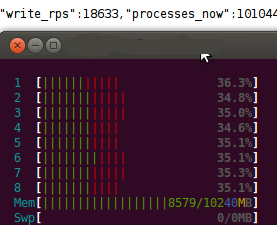
\includegraphics[width=.5\textwidth]{top.png}
  \end{center}
\end{frame}

\begin{frame}{YAWNDB: ссылки}
  \begin{itemize}
  \item Graphite \url{https://github.com/graphite-project}
  \item Ecirca \url{https://github.com/band115/ecirca}
  \item Cowboy \url{https://github.com/extend/cowboy}
  \item Cowboy \url{https://github.com/uwiger/gproc}
  \item McErlang \url{https://github.com/fredlund/McErlang}
  \end{itemize}
\end{frame}

\begin{frame}
  \begin{center}
    \Large
    Облака
  \end{center}
\end{frame}

\begin{frame}[plain]
  \begin{tikzpicture}[remember picture,overlay]
    \node[at=(current page.center)] {
      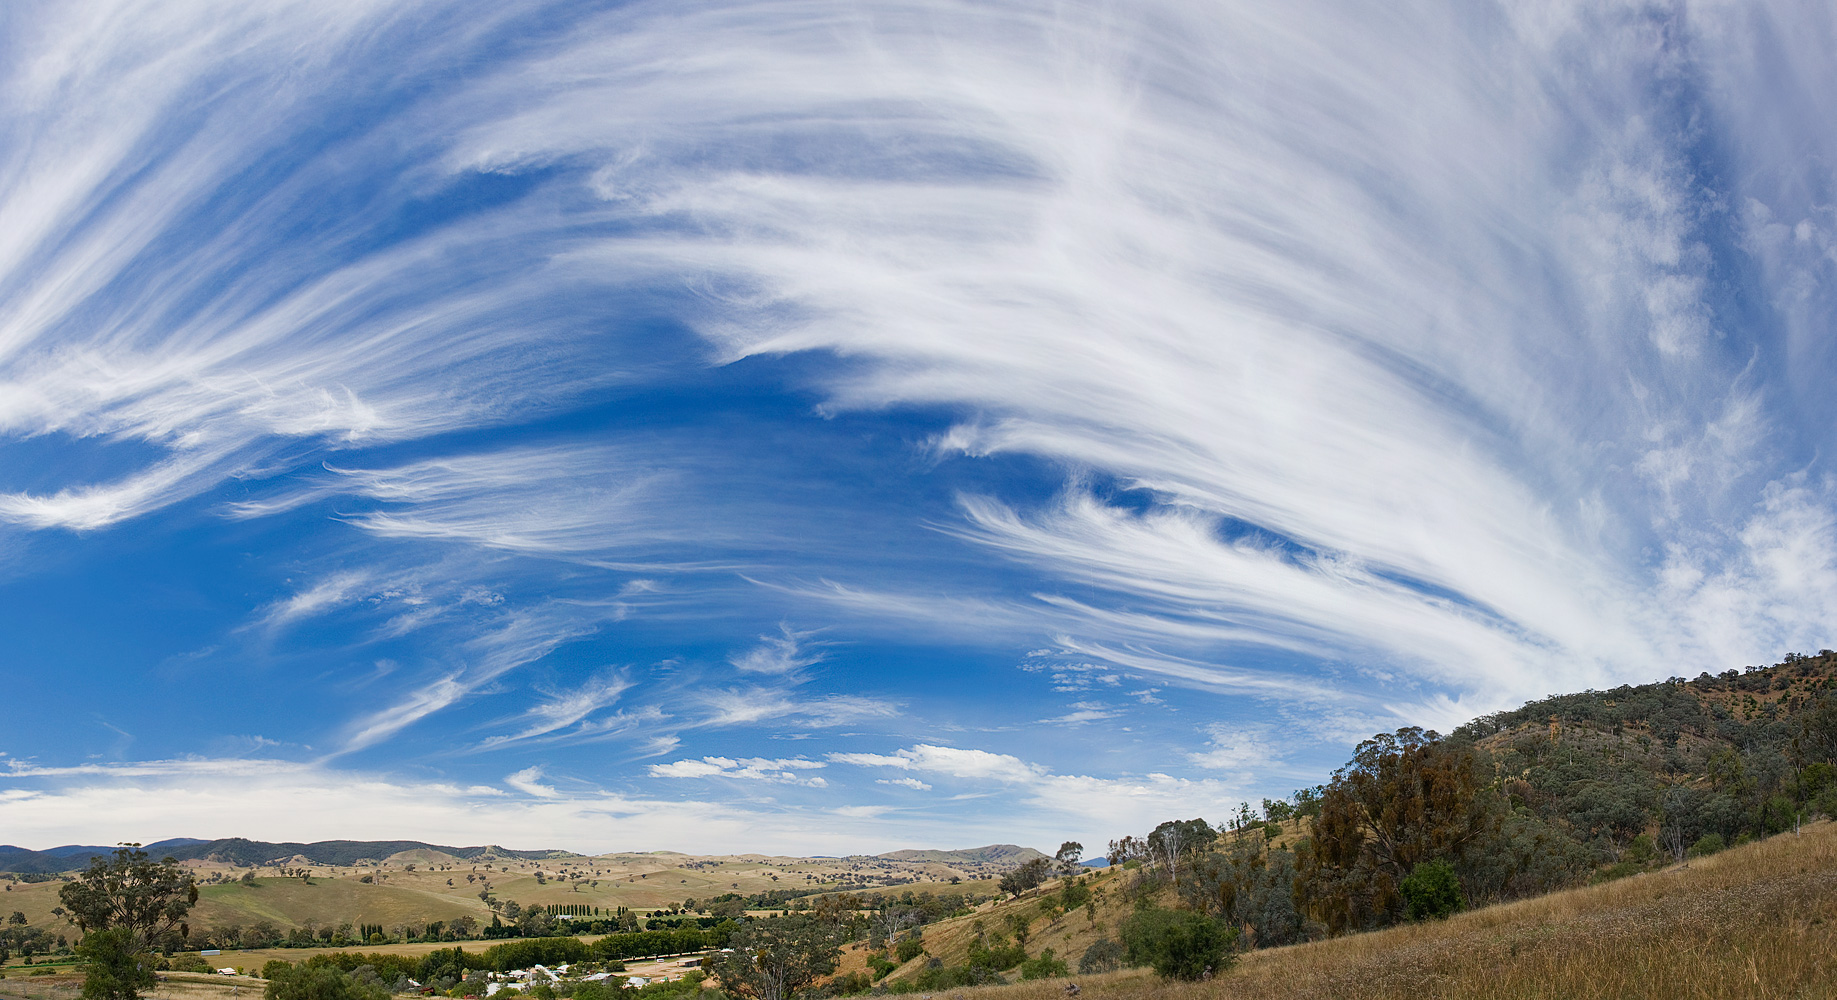
\includegraphics[height=\paperheight]{clouds.jpg}
    };
  \end{tikzpicture}
\end{frame}

\begin{frame}{Об облаках}
  Xen:
  \begin{itemize}
  \item Dom0, DomU
  \item запуск и остановка доменов
  \item простой и неубиваемый
  \end{itemize}
  XAPI (XenAPI) от Citrix:
  \begin{itemize}
  \item Миграция
  \item Пулы
  \item Динамическое управление памятью
  \item ...
  \end{itemize}
\end{frame}

\begin{frame}{Больше, чем XAPI}
  \begin{itemize}
  \item учёт используемых ресурсов (биллинг, статистика)
  \item управление машинами из биллинга, веб-интерфейса, API и администраторами
  \item детекция нештатных ситуаций (падение хранилища либо сети)
  \item динамическая балансировка нагрузки
  \item предоставление интерфейсов к машине, не предусмотренных XAPI
    (web-консоль, realtime потребление, MemoryOnDemand)
  \end{itemize}
  Много сложной «бизнес»-логики
\end{frame}

\begin{frame}{Старая архитектура}
  \begin{itemize}
    \item {\bf Make it work}, make it right, make it fast
    \item Python+Bash помойка
    \item Коммуникация через HTTP, Mongo и redis (aka «как получится»)
    \item WTF is summationd? WTF is yawndbtiond-obsolete?
    \item боль с Python+Mongo — много раздельного кода, размазывание схемы
  \end{itemize}
\end{frame}

\begin{frame}{Новая архитектура}
  \begin{itemize}
    \item Make it work, {\bf make it right}, make it fast
    \item Построение «от API»
    \item VBD/VDI/VIF/BDSM → Disk/Network interface/...
    \item Фиксированная схема данных
    \item Erlang для сети и рантайма, Haskell для «бизнес»-логики
    \item Механизм Erlang ports — stdin/stdout + Erlang External Term Format
  \end{itemize}
\end{frame}

\begin{frame}{Новая архитектура}
  \begin{tikzpicture}[node distance=1cm, auto,]
    \node[actor] (rnbwdash) {Rainbow Dash};
    \node[actor, left=0.9cm of rnbwdash] (client) {Happy customer}
    edge[arr, <->] (rnbwdash);
    \node[actor, right=0.9cm of rnbwdash] (twlght1) {Twilight Sparkle}
    edge[arr, <->] (rnbwdash);
    \node[actor, above=0.3cm of twlght1] (twlght2) {Twilight Sparkle}
    edge[arr, <->] (rnbwdash);
    \node[actor, below=0.3cm of twlght1] (twlght3) {Twilight Sparkle}
    edge[arr, <->] (rnbwdash);
    \node[actor, right=1.5cm of twlght1] (mongo) {Legacy Mongo}
    edge[arr, <->] (twlght1.east)
    edge[arr, <->] (twlght2.east)
    edge[arr, <->] (twlght3.east);
    \node[actor, above=1cm of mongo] (postgre) {PostgreSQL}
    edge[arr, <->, bend right=5] (twlght1.east)
    edge[arr, <->, bend right=10] (twlght2.east)
    edge[arr, <->, bend right=20] (twlght3.east);
    \node[actor, below=1cm of mongo] (xapi) {XAPI}
    edge[arr, <->, bend left=20] (twlght1.east)
    edge[arr, <->, bend left=10] (twlght2.east)
    edge[arr, <->, bend left=5] (twlght3.east);
  \end{tikzpicture}
\end{frame}

\begin{frame}
  \begin{center}
    \Large
    Rainbowdash
  \end{center}
\end{frame}

\begin{frame}[plain]
  \begin{tikzpicture}[remember picture,overlay]
    \node[at=(current page.center)] {
      
\includegraphics[height=\paperheight]{rainbowdash.jpg}
    };
  \end{tikzpicture}
\end{frame}

\begin{frame}{Rainbowdash}
  \begin{itemize}
    \item Милая, быстрая, немного простоватая, но reliable для друзей
    \item REST + RPC: HTTP REST API → RPC API на фронтенде по конфигу с верификацией (type safety!)
    \item Асинхронность + синхронность: интерфейс синхронный, rainbowdash асинхронна, twilightsparkle синхронна
    \item «Задачи» с уникальным идентификатором для каждого запроса
    \item 2-phase commit задачи: проверка корректности и ожидаемой ресурсоёмкости, запуск (возможно, отложенный)
    \item балансировка нагрузки на бекендах по ожидаемым ресурсам и внешним характеристикам процессов (ping, mem)
    \item отчёты о состоянии системы (ping, mem, cpu, rps, latency)
    \item 2-phase commit конфига
    \item почти live reloading Haskell-кода с персистентными задачами и HTTP-коннектами
  \end{itemize}
\end{frame}

\begin{frame}{Rainbowdash: выводы}
  \begin{itemize}
  \item переход программистов Python → Erlang занимает неделю-полторы
  \item запаковка не-Erlang кода с помощью rebar это боль (Make+bash+cabal+cabal-dev)
  \item jobs — прекрасная библиотека, но документации почти нет
  \item любить себя полезно, несколько часов на автоматизацию перезагрузки бекенда при изменении бинарника окупились многократно
  \item кода до первой работоспособной версии достаточно мало (1k строк)
  \end{itemize}
\end{frame}

\begin{frame}{Rainbowdash: ссылки}
  \begin{itemize}
  \item jobs \url{https://github.com/uwiger/jobs/}
  \end{itemize}
\end{frame}

\begin{frame}
  \begin{center}
    \Large
    Twilightsparkle
  \end{center}
\end{frame}

\begin{frame}[plain]
  \begin{tikzpicture}[remember picture,overlay]
    \node[at=(current page.center)] {
      
\includegraphics[height=\paperheight]{twilight.png}
    };
  \end{tikzpicture}
\end{frame}


\begin{frame}{TwiligthSparkle}
\begin{itemize}
  \item Общая архитектура
  \item Template Haskell и генерация сервера
  \item Контроль ошибок на уровне типов
  \item Барьеры — откат изменений
  \item Persistent ORM
  \item Проблемы при разработке
\end{itemize}
\end{frame}

\begin{frame}[fragile]{TwiligthSparkle: общая архитектура}
\begin{itemize}
  \item Сервер, занимающийся чтением запросов из stdin и пишущий ответы
  в stdout
  \item Используется стандартный для Эрланга способ коммуникации — порты
  \begin{itemize}
    \item Был написан модуль реализующий ETF (External Term Format)
  \end{itemize}
  \item Воркеры, выполняющиеся в отдельных процессах
  \item Сложное ядро, максимально простой API для написания непосредственно
  обработчиков запросов
  \item Каждый запрос определяется тремя параметрами: source, input и result
  \begin{itemize}
    \item source — Источник задачи, в нашем случае это пользователь API,
    администратор или внутренний сервис
    \item input — Входные данные запроса
    \item result — Результат на выполнение запроса
  \end{itemize}
  \begin{minted}[fontsize=\footnotesize]{haskell}
    class TaskSource source => Task source input result
  \end{minted}
\end{itemize}
\end{frame}

\begin{frame}[fragile]{TwiligthSparkle: Template Haskell и генерация сервера}

  Template Haskell используется для генерации функций разбора запросов
  от сервера. Например из кода:

  \begin{minted}[fontsize=\footnotesize]{haskell}
    [erlServer|
        vm_start :: TS User VMStartTask ()
    |]
  \end{minted}

генерируется код:

  \begin{minted}[fontsize=\footnotesize]{haskell}
  dispatch ref "vm_start"
           (ErlTuple [ErlBinary "user", ErlInt userId])
           inputV = case fromErl inputV of
      Nothing -> invalidTask
      Just (i :: VMStartTask) -> do
          ...  -- Process request
  dispatch ref "vm_start" _user _input = invalidTask
\end{minted}
\end{frame}

\begin{frame}[fragile]{TwiligthSparkle: Контроль ошибок}

  \begin{itemize}
    \item Прерывание выполнения подобно ErrorT трансформеру
    \item Отдельные типы для каждого вида ошибок
    \item Требование явного декларирования списка возможных ошибок
    \end{itemize}
  \begin{minted}[fontsize=\footnotesize]{haskell}
    instance AllowError source VMStartTask () VMNotFound
    instance AllowError source VMStartTask () VMIsAlreadyRunning
  \end{minted}
  \begin{itemize}
    \item Пока нет, но хочется контроль декларированных и не вызываемых ошибок
  \end{itemize}
\end{frame}

\begin{frame}[fragile]{TwiligthSparkle: Барьеры}

  \begin{itemize}
    \item Существует необходимость отката изменений в случае ошибок
    \item Барьеры устанавливаются после изменения, для которого требуется откат
     и выполняются в случае возникновения ошибки
  \end{itemize}
  \begin{minted}[fontsize=\footnotesize]{haskell}
    vm <- createVm
    barrier $ destroyVm vm
    disk <- createDisk
    barrier $ destroyDisk disk
    error "Any error"
  \end{minted}
  \begin{itemize}
    \item Технически реализовано как [TS source input result ()]
     внутри TVar контекста ReaderT
  \end{itemize}

\end{frame}

\begin{frame}[fragile]{TwiligthSparkle: Persistent ORM}
  \begin{itemize}
    \item Первая версия не использовала ORM
  \end{itemize}
  \begin{minted}[fontsize=\footnotesize]{haskell}
    vm@(VM { vmUuid, vmTemplate }) <-
        fetch VMCollection [ "id" =: iVmId ]
  \end{minted}
  \begin{itemize}
    \item Регулярно возникали опечатки в названиях полей, в передаваемых данных
    \item Для Хаскеля нет рабочих альтернативных ORM кроме persistent
  \end{itemize}
  \begin{minted}[fontsize=\footnotesize]{haskell}
    vm@(VM { vmUuid, vmTemplate }) <- fetch [ VmId ==. iVmId ]
  \end{minted}
  \begin{itemize}
    \item Пришлось использовать патченную версию persistent-mongodb, так как
    модель хранения отличается от подразумеваемой разработчиками
  \end{itemize}
\end{frame}

\begin{frame}{TwiligthSparkle: Проблемы при разработке}
  \begin{itemize}
    \item Space leaks
    \begin{itemize}
      \item Очень трудно найти источник проблемы при большом объёме кода
    \end{itemize}
    \item Не хватает некоторых пакетов на hackage, либо не устраивает их состояние
    \begin{itemize}
      \item Написали библиотеку для работы с ETF
      \item Стали поддерживать библиотеки bson и mongoDB
    \end{itemize}
    \item Вероятно, более высокий порог вхождения
    \begin{itemize}
      \item Тем не менее в проект, кроме ядра, успешно пишут программисты
      без какого-либо функционального бэкграунда
    \end{itemize}
  \end{itemize}
\end{frame}

% \begin{frame}{TwiligthSparkle: Выводы}
%   \begin{itemize}
%     \item Заметно упало количество не логических ошибок, например:
%     \begin{itemize}
%       \item Параметризованные идентификаторы, например (UUID VM), не допускают
%       их использование для не VM объектов
%     \end{itemize}
%     \item Template Haskell — позволяет удобно решать проблемы, но
%     катастрофически плохо читается
%   \end{itemize}
% \end{frame}

\begin{frame}
  \begin{center}
    \Large
    Вопросы?
  \end{center}
\end{frame}

\begin{frame}\label{lastframe}
  Copyrighted stuff:
  \footnotesize
  \url{https://en.wikipedia.org/wiki/File:Cirrus\_sky\_panorama.jpg} \\
  \url{http://www.wallpapervortex.com/wallpaper-15684\_1\_other\_wallpapers\_my\_little\_pony.html} \\
  \url{http://www.tikihumor.com/3287/rainbow-dash-makes-it-rain/rainbow-dash-makes-it-rain-2/}
  \url{http://qeinone.deviantart.com/art/Twilight-Sparkle-205789859}
\end{frame}